%-------------------------------------------------
%	Version: 0.0
%	fecha de entrega
%
%-------------------------------------------------

\documentclass[11pt]{report}

%packages
\usepackage{graphicx}
\usepackage{subcaption}

\usepackage[utf8]{inputenc}
\usepackage[spanish, es-nodecimaldot]{babel}
\usepackage{setspace}
\usepackage{ragged2e}

\usepackage{amsmath}
\usepackage{amsthm}
\usepackage{amssymb}
\usepackage{mathtools}
\usepackage{siunitx}
\usepackage[thinc]{esdiff} %derivadas faciles
\usepackage{physics} %algunos simbolos de derivadas

%path donde se encuentran las imagenes
\graphicspath{ {./figuras/} }

%---------------------------------------------------------------
%ABREVIACIONES DE COMANDOS

\theoremstyle{plain}
\newtheorem{thm}{Teorema}[chapter] % reset theorem numbering for each chapter

\theoremstyle{definition}
\newtheorem{defn}[thm]{Definición} % definition numbers are dependent on theorem numbers
\newtheorem{exmp}[thm]{Ejemplo} % same for example numbers

\newcommand{\chaptercontent}{
\section{Basics}
\begin{defn}Here is a new definition.\end{defn}
\begin{thm}Here is a new theorem.\end{thm}
\begin{thm}Here is a new theorem.\end{thm}
\begin{exmp}Here is a good example.\end{exmp}
\subsection{Some tips}
\begin{defn}Here is a new definition.\end{defn}
\section{Advanced stuff}
\begin{defn}Here is a new definition.\end{defn}
\subsection{Warnings}
\begin{defn}Here is a new definition.\end{defn}
}

\usepackage{biblatex}
%\addbibresource{Tarea1.bib}

\begin{document}

\begin{titlepage}
\title{Titulo_del_trabajo}

%-------------------------------------------------
%PORTADA
%-------------------------------------------------

	\centering
	{\scshape\LARGE Universidad Autónoma de Yucatán  \\ Facultad de ingeniería\par}
	\vspace{1cm}
	{\scshape\Large Teoría electromagnética 2\par}
	\vspace{1.5cm}
	{\huge\bfseries ADA 1 Ensayo, corrientes eléctricas\par}
	\vspace{0.7cm}
	{\begin{figure}[!h]
	\centering
    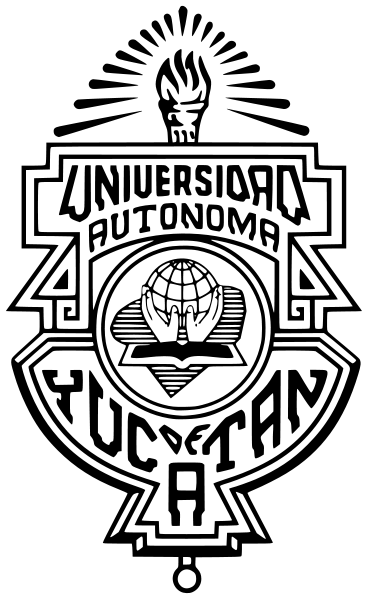
\includegraphics[scale=0.3]{UADY.png}
	\end{figure}}
	\vspace{0.7cm}
	{\Large\itshape Erick Al. Casanova Cortés\par}
	{\Large\itshape Matricula: 15014866\par}
	\vfill
	{\scshape\Large Docente\par
	Dr. O. Carvente\par}
	\vfill
	{\Large{\bfseries Fecha de entrega: 8 Marzo 2021} }

	\vfill
	
\end{titlepage}

%-------------------------------------------------
%Inicio del documento
%-------------------------------------------------


%-------------------------------------------------
%Instrucciones
\section*{Instrucciones}
Resolver de modo numérico con ayuda de algún software el siguiente ejercicio:

%-------------------------------------------------
%Planteamiento
\section*{Ejercicio}

	Corrientes, encontrar la fuerza que $I'$ ejerce sobre $I$.
	
	Partiendo de (\ref{eq:ley_ampere}), tenemos que definir los vectores que vamos a utilizar, los cuales serán
	
	
	\begin{figure}[!h]%grafico
		\centering
		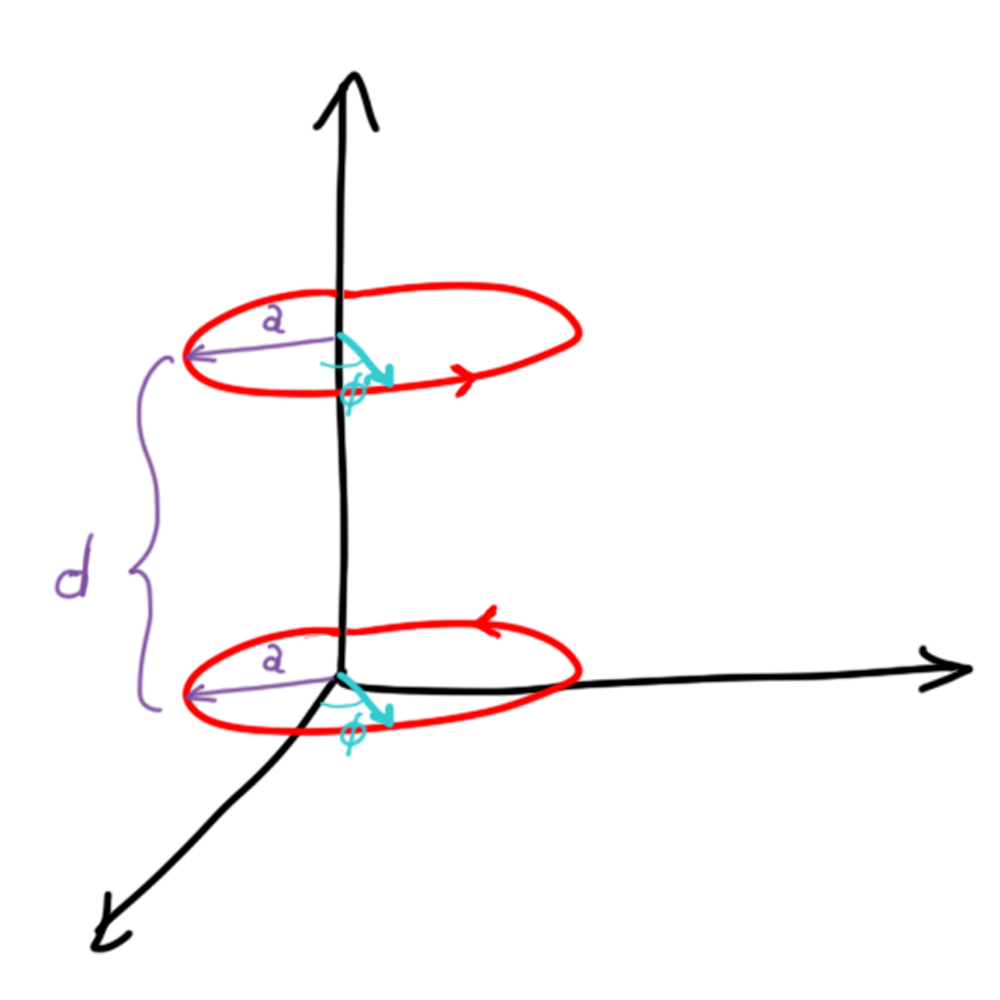
\includegraphics[scale=0.15]{Tarea2_figura.png}
		\caption{Dos circuitos}
		\label{fig:Tarea2}
	\end{figure}
	
	\begin{align*}%vectores de posición
		\vec{r}' &= a\cos\varphi'\hat{i} + a\sin\varphi'\hat{j}\\
		\vec{r} &= a\cos\varphi\hat{i} + a\sin\varphi\hat{j}+d\hat{k}\\
	\end{align*}
	
	\begin{align*}%diferencia de vectores
		\vec{r} - \vec{r}' &= a\cos\varphi\hat{i} + a\sin\varphi\hat{j}+d\hat{k} - (a\cos\varphi'\hat{i} + a\sin\varphi'\hat{j})\\
		&= a(\cos\varphi-\cos\varphi')\hat{i} + a(\sin\varphi-\sin\varphi')\hat{j} + d\hat{k}
	\end{align*}
	
	\begin{align*}%modulo de la diferencia de vectores
		|\vec{r} - \vec{r}'| &= \sqrt{a^2(\cos\varphi-\cos\varphi')^2 + a^2(\sin\varphi-\sin\varphi')^2 + d^2}
	\end{align*}
	
	\begin{align*}%diferenciales
		\dd{s'} &= a \left(-\sin\varphi'\hat{i} + \cos\varphi'\hat{j}\right)\dd{\varphi'}\\
		\dd{s} &= a \left(-\sin\varphi\hat{i} + \cos\varphi\hat{j}\right)\dd{\varphi}
	\end{align*}
	
	Entonces la fuerza que ejerce $C$ sobre $C'$ es

	\begin{align*}%integral a resolver
		\vec{F}_{C'\rightarrow C}&= \frac{\mu_0}{4\pi}\int_0^{2\pi}\int_0^{2\pi} a \left(-\sin\varphi\hat{i} + a\cos\varphi\hat{j}\right)\dd{\varphi} \times \left[ a \left(-\sin\varphi'\hat{i} + \cos\varphi'\hat{j}\right)\dd{\varphi'} \times \frac{(\vec{r} - \vec{r}')}{|\vec{r} - \vec{r}'|^3}\right]
	\end{align*}
	
	
	Para resolver esta integral se opto por utilizar python, antes de meterla al programa hay que hacerle un tratamiento, como principio, podemos ver que $a$ es una constante, por lo que podemos reescribir la ecuación como
	
	\begin{align*}%integral a resolver
		\vec{F}_{C'\rightarrow C}&= \frac{\mu_0a^2}{4\pi}\int_0^{2\pi}\int_0^{2\pi}\left(-\sin\varphi\hat{i} + \cos\varphi\hat{j}\right)\dd{\varphi} \times \left[  \left(-\sin\varphi'\hat{i} + \cos\varphi'\hat{j}\right)\dd{\varphi'} \times \frac{(\vec{r} - \vec{r}')}{|\vec{r} - \vec{r}'|^3}\right]
	\end{align*}

	Analizando el producto cruz $\left(-\sin\varphi'\hat{i} + \cos\varphi'\hat{j}\right)\dd{\varphi'} \times \frac{(\vec{r} - \vec{r}')}{|\vec{r} - \vec{r}'|^3}$, sustituyendo los valores podemos ver que
	
	\begin{equation*}%cuz
		\left(-\sin\varphi'\hat{i} + \cos\varphi'\hat{j}\right)\dd{\varphi'} \times \frac{a(\cos\varphi-\cos\varphi')\hat{i} + a(\sin\varphi-\sin\varphi')\hat{j} + d\hat{k}}{\left(a^2(\cos\varphi-\cos\varphi')^2 + a^2(\sin\varphi-\sin\varphi')^2 + d^2\right)^{3/2}}
	\end{equation*}
	
	Analizando solo la parte vectorial
	
	\begin{equation*}
		\left(-\sin\varphi'\hat{i} + \cos\varphi'\hat{j}\right) \times \left[a(\cos\varphi-\cos\varphi')\hat{i} + a(\sin\varphi-\sin\varphi')\hat{j} + d\hat{k} \right]
	\end{equation*}
	
	Expandiendo usando distributividad
	
	\begin{align*}%distrib
		\left(-\sin\varphi'\hat{i} + \cos\varphi'\hat{j}\right) \times \left[a(\cos\varphi-\cos\varphi')\hat{i} + a(\sin\varphi-\sin\varphi')\hat{j} + d\hat{k} \right] =\\
		-\sin\varphi'*a(\cos\varphi-\cos\varphi')\left(\hat{i}\times\hat{i}\right) -\sin\varphi'*a(\sin\varphi-\sin\varphi') \left(\hat{i}\times\hat{j}\right) -\sin\varphi'*d \left(\hat{i}\times\hat{k}\right) \\
		+\cos\varphi'*a(\cos\varphi-\cos\varphi') \left(\hat{j}\times\hat{i}\right) + \cos\varphi'*a(\sin\varphi-\sin\varphi') \left(\hat{j}\times\hat{j}\right) + \cos\varphi'*d\left(\hat{j}\times\hat{k}\right)
	\end{align*}
	
	Es evidente que algunos de estos términos se anularán, quedándonos como:
	
	\begin{align*}%evaluando producto vectorial
		\left(-\sin\varphi'\hat{i} + \cos\varphi'\hat{j}\right) \times \left[a(\cos\varphi-\cos\varphi')\hat{i} + a(\sin\varphi-\sin\varphi')\hat{j} + d\hat{k} \right] =\\
		-\sin\varphi'*a(\sin\varphi-\sin\varphi')\hat{k} + d\sin\varphi'\hat{j} \\
		-\cos\varphi'*a(\cos\varphi-\cos\varphi')\hat{k} + d\cos\varphi'\hat{i}
	\end{align*}
	
	Agrupando términos semejantes:
	
	\begin{align*} % agrupando
		\left(-\sin\varphi'\hat{i} + \cos\varphi'\hat{j}\right) \times \left[a(\cos\varphi-\cos\varphi')\hat{i} + a(\sin\varphi-\sin\varphi')\hat{j} + d\hat{k} \right] =\\
		d\cos\varphi'\hat{i}+d\sin\varphi'\hat{j}-a\left(\sin\varphi'\sin\varphi+\cos\varphi'\cos\varphi-\cos^2\varphi'-\sin^2\varphi'\right)\hat{k}
	\end{align*}
	
	Podemos identificar dos identidades trigonométricas en esta ecuación
	
	\begin{align*}% identidades trigonometricas
		\sin^2{\theta} + \cos^2{\theta} &= 1\\
		\cos{\alpha - \beta} &= \sin{\alpha }\sin{\beta}+\cos{\alpha }\cos{\beta}
	\end{align*}
	
	Por lo que nos queda la expresión como:
	
	\begin{align*} % sustitucion
		\left(-\sin\varphi'\hat{i} + \cos\varphi'\hat{j}\right) \times \left[a(\cos\varphi-\cos\varphi')\hat{i} + a(\sin\varphi-\sin\varphi')\hat{j} + d\hat{k} \right] =\\
		d\cos\varphi'\hat{i}+d\sin\varphi'\hat{j}-a\left[\cos{(\varphi-\varphi')}-1\right]\hat{k}
	\end{align*}
	
	Regresando a la expresión dentro de la integral:
	\begin{align*}%integral a resolver
		\vec{F}_{C'\rightarrow C}&= \frac{\mu_0a^2}{4\pi}\int_0^{2\pi}\int_0^{2\pi}\frac{\left(-\sin\varphi\hat{i} + \cos\varphi\hat{j}\right)\dd{\varphi} \times d\cos\varphi'\hat{i}+d\sin\varphi'\hat{j}-a\left[\cos{(\varphi-\varphi')}-1\right]\hat{k}}{\left(a^2(\cos\varphi-\cos\varphi')^2 + a^2(\sin\varphi-\sin\varphi')^2 + d^2\right)^{3/2}}\dd{\varphi'}
	\end{align*}
	
	Volviendo a hacer un análisis de las componentes vectoriales
	
	\begin{align*}%parte vectorial
		\left(-\sin\varphi\hat{i} + \cos\varphi\hat{j}\right)\dd{\varphi} \times d\cos\varphi'\hat{i}+d\sin\varphi'\hat{j}-a\left[\cos{(\varphi-\varphi')}-1\right]\hat{k}\\
	\end{align*}
	
	Aplicando de nuevo distributividad
	
	\begin{align*}%parte vectorial distrib
		\left(-\sin\varphi\hat{i} + \cos\varphi\hat{j}\right)\dd{\varphi} \times d\cos\varphi'\hat{i}+d\sin\varphi'\hat{j}-a\left[\cos{(\varphi-\varphi')}-1\right]\hat{k} = \\
		-d\sin\varphi \cos\varphi'\hat{i} * \hat{i} -d\sin\varphi\sin\varphi'\hat{i}*\hat{j}+ a\sin\varphi\left[\cos{(\varphi-\varphi')}-1\right]\hat{i}*\hat{k}\\
		+d\cos\varphi\cos\varphi'\hat{j}*\hat{i} + d\cos\varphi\sin\varphi'\hat{j}*\hat{j} - a\cos\varphi\left[\cos{(\varphi-\varphi')}-1\right]\hat{j}*\hat{k}
	\end{align*}
	
	Lo que nos queda de la siguiente manera
	
	\begin{align*}%parte vectorial eval
		\left(-\sin\varphi\hat{i} + \cos\varphi\hat{j}\right)\dd{\varphi} \times d\cos\varphi'\hat{i}+d\sin\varphi'\hat{j}-a\left[\cos{(\varphi-\varphi')}-1\right]\hat{k} = \\
		- d\sin\varphi\sin\varphi'\hat{k} - a\sin\varphi\left[\cos{(\varphi-\varphi')}-1\right]\hat{j}\\
		-d\cos\varphi\cos\varphi'\hat{k} - a\cos\varphi\left[\cos{(\varphi-\varphi')}-1\right]\hat{i}
	\end{align*}
	
	Agrupando términos semejantes
	
	\begin{align*}%agrupando
		\left(-\sin\varphi\hat{i} + \cos\varphi\hat{j}\right)\dd{\varphi} \times d\cos\varphi'\hat{i}+d\sin\varphi'\hat{j}-a\left[\cos{(\varphi-\varphi')}-1\right]\hat{k} = \\
		- a\cos\varphi\left[\cos{(\varphi-\varphi')}-1\right]\hat{i} - a\sin\varphi\left[\cos{(\varphi-\varphi')}-1\right]\hat{j}
		- d\left( \sin\varphi\sin\varphi'+\cos\varphi\cos\varphi'\right)\hat{k} 
	\end{align*}
	
	Retomando una de las igualdades trigonométricas vistas con anterioridad: 
	
	\begin{align*}%trig
		\left(-\sin\varphi\hat{i} + \cos\varphi\hat{j}\right)\dd{\varphi} \times d\cos\varphi'\hat{i}+d\sin\varphi'\hat{j}-a\left[\cos{(\varphi-\varphi')}-1\right]\hat{k} = \\
		- a\cos\varphi\left[\cos{(\varphi-\varphi')}-1\right]\hat{i} - a\sin\varphi\left[\cos{(\varphi-\varphi')}-1\right]\hat{j}
		- d\cos{(\varphi - \varphi')}\hat{k} 
	\end{align*}
	
	Regresando a la integral:
	
	\begin{align*}%integral a resolver
		\vec{F}_{C'\rightarrow C} &= \frac{\mu_0a^2}{4\pi}\int_0^{2\pi}\int_0^{2\pi}\frac{ - a\cos\varphi\left[\cos{(\varphi-\varphi')}-1\right]\hat{i} }{\left(a^2(\cos\varphi-\cos\varphi')^2 + a^2(\sin\varphi-\sin\varphi')^2 + d^2\right)^{3/2}}\dd{\varphi}\dd{\varphi'}\\
		&+ \frac{\mu_0a^2}{4\pi}\int_0^{2\pi}\int_0^{2\pi}\frac{ - a\sin\varphi\left[\cos{(\varphi-\varphi')}-1\right]\hat{j} }{\left(a^2(\cos\varphi-\cos\varphi')^2 + a^2(\sin\varphi-\sin\varphi')^2 + d^2\right)^{3/2}}\dd{\varphi}\dd{\varphi'}\\
		&+ \frac{\mu_0a^2}{4\pi}\int_0^{2\pi}\int_0^{2\pi}\frac{ - d\cos{(\varphi - \varphi')}\hat{k}  }{\left(a^2(\cos\varphi-\cos\varphi')^2 + a^2(\sin\varphi-\sin\varphi')^2 + d^2\right)^{3/2}}\dd{\varphi}\dd{\varphi'}
	\end{align*}
	
	Las tres integrales que nos quedan son mucho más fáciles de programar
%-------------------------------------------------
%Final del documento
%-------------------------------------------------

\end{document}
